% AAAI 2026 Submission
% Risk-Calibrated Test-Time Decision Making for Reliable RAG
\documentclass[letterpaper]{article}
\usepackage{aaai2026}  % AAAI 2026 style
\usepackage{times}
\usepackage{helvet}
\usepackage{courier}
\usepackage[hyphens]{url}
\usepackage{graphicx}
\urlstyle{rm}
\sloppy
\emergencystretch=3em
\usepackage{algorithm}
\usepackage{algorithmic}
\usepackage{booktabs}
\usepackage{amsmath}
\usepackage{amssymb}
\usepackage{amsthm}
\usepackage{multirow}
\usepackage{xcolor}

\pdfinfo{
/TemplateVersion (2026.1)
}

% Disable comments for submission
\nocopyright

% Algorithm package settings
\renewcommand{\algorithmicrequire}{\textbf{Input:}}
\renewcommand{\algorithmicensure}{\textbf{Output:}}

% Theorem environments
\newtheorem{theorem}{Theorem}
\newtheorem{lemma}{Lemma}
\newtheorem{proposition}{Proposition}

\title{Risk-Calibrated Test-Time Decision Making for Reliable Retrieval-Augmented Generation}
\author{Anonymous}
\affiliations{Paper ID XXX}

\begin{document}
\maketitle

\begin{abstract}
Retrieval-Augmented Generation (RAG) improves factual grounding in Large Language Models (LLMs) but does not guarantee reliability: retrieved evidence may be irrelevant, contradictory, or misleading, leading to confident errors. Existing approaches treat uncertainty quantification and abstention separately, offering only binary answer-or-abstain decisions. We formalize the \emph{RAG test-time risk control} problem with four actions---\textsc{Answer}, \textsc{RetrieveMore}, \textsc{VerifyMore}, and \textsc{Abstain}---under a limited compute budget, and propose \textbf{RC-TTD} (Risk-Calibrated Test-Time Decision Policy), a two-stage method combining conformal prediction with a retrieval-aware nonconformity score. Stage~1 uses answer probability ($1{-}p_{\max}$) for conformal coverage ($\geq 1{-}\alpha$), while Stage~2 leverages a multi-signal score---fusing answer uncertainty, retrieval relevance, evidence conflict, answer-evidence support, and verifier disagreement---to select corrective actions. We prove five theoretical results: (1) marginal score coverage, (2) a formal \emph{score distribution compression} lemma with explicit assumptions showing why naive combined-score calibration fails, (3) a selective risk decomposition theorem, (4) a cost-optimality theorem over general single-action policies, and (5) a risk-coverage trade-off theorem showing strict risk improvement at matched coverage. We also formally characterize the \emph{confident error} limitation. Experiments on SciQ, SciFact, and wrong-context stress tests with LLaMA-3.1-8B use \emph{real end-to-end corrective actions} (re-retrieval with top-15, per-evidence NLI-weighted verification), showing RC-TTD maintains target coverage ($\sim$90\%), achieves strictly lower selective risk than probability-only abstention at matched coverage, and provides provably better cost-risk trade-offs. Under wrong-context corruption, where LAC/APS become over-conservative (coverage drops to 0.81), RC-TTD maintains \textbf{$\sim$100\% coverage} with \textsc{RetrieveMore} fix rates up to 36\%.
\end{abstract}

%==========================================================================
\section{Introduction}
%==========================================================================

Retrieval-Augmented Generation (RAG)~\cite{lewis2020rag,gao2024retrieval} has become the standard approach for grounding Large Language Model (LLM) outputs in external knowledge, reducing hallucinations~\cite{ji2023survey,shuster2021retrieval} by incorporating retrieved evidence at inference time. However, RAG systems are not inherently reliable: the retrieval pipeline may return irrelevant documents, the evidence may be contradictory, or the model may be misled by plausible-but-incorrect context. These failure modes produce \emph{confident errors}---cases where the model generates a wrong answer with high confidence~\cite{kadavath2022language,mallen2023not}---which are particularly dangerous in high-stakes domains such as healthcare, science, and finance. Compounding this, recent work~\cite{schaeffer2024are} shows that such confident errors are not rare tail events but systematic failure modes under distribution shift.

Existing approaches to RAG reliability fall into three lines of work, each with limitations. First, \textbf{uncertainty quantification} benchmarks like URAG \cite{ye2025urag} systematically evaluate RAG confidence calibration but do not prescribe what action to take when uncertainty is high; similarly, language-model self-knowledge studies \cite{kadavath2022language,lin2022teaching,tian2023just,kuhn2023semantic} provide richer confidence signals but stop short of decision-making. Second, \textbf{conformal abstention} methods \cite{mohri2024conformal,quach2024conformal,sadinle2019least,romano2020classification} provide distribution-free risk guarantees \cite{vovk2005algorithmic,angelopoulos2023conformal} but are limited to binary answer-or-abstain decisions, ignoring RAG-specific corrective actions such as retrieving additional evidence or verifying the answer against multiple sources. Third, \textbf{test-time compute scaling} research \cite{snell2024solve,lightman2023let} studies how to allocate additional computation between solving and verifying, but does not address RAG-specific signals like retrieval relevance or evidence conflict, nor does it provide calibrated risk control.

The key insight of this paper is that RAG systems benefit from a \emph{multi-action} decision framework that goes beyond binary abstention. When a RAG system is uncertain about an answer, the appropriate response depends on \emph{why} it is uncertain: if retrieval is irrelevant, the system should retrieve more evidence; if evidence is contradictory, it should verify the answer; if the model is fundamentally unsure even with good evidence, it should abstain. This requires a risk-calibrated policy that maps the RAG system's internal signals to one of four actions under a limited compute budget.

We formalize this as the \emph{RAG test-time risk control} problem and propose \textbf{RC-TTD} (Risk-Calibrated Test-Time Decision Policy), a two-stage method that decouples conformal coverage guarantees from corrective action selection. Figure~\ref{fig:overview} illustrates the overall pipeline. Our main contributions are:

\begin{enumerate}
    \item \textbf{Problem formulation:} We define the RAG test-time multi-action risk control problem with four actions (\textsc{Answer}, \textsc{RetrieveMore}, \textsc{VerifyMore}, \textsc{Abstain}) under a compute budget, incorporating RAG-specific signals.

    \item \textbf{Retrieval-aware nonconformity score:} We design a multi-signal score fusing five uncertainty diagnostics and demonstrate through ablation that each signal contributes to risk prediction quality.

    \item \textbf{Theoretical analysis with five results:} We prove (i) marginal score coverage (Theorem~\ref{thm:coverage}), (ii) a \emph{score distribution compression lemma} (Lemma~\ref{lem:compression}) with explicit assumptions, (iii) a \emph{selective risk decomposition theorem} (Theorem~\ref{thm:risk}), (iv) a \emph{cost-optimality theorem} (Theorem~\ref{thm:cost}) over general single-action policies, and (v) a \emph{risk-coverage trade-off theorem} (Theorem~\ref{thm:tradeoff}) showing strict risk improvement at matched coverage. We also formally characterize the \emph{confident error} limitation (Proposition~\ref{prop:confident}).

    \item \textbf{Empirical validation with real corrective actions:} We evaluate RC-TTD on SciQ, SciFact, and wrong-context stress tests with LLaMA-3.1-8B-Instruct using \emph{real end-to-end corrective actions} (re-retrieval with top-15, per-evidence NLI-weighted verification). RC-TTD maintains target coverage ($\sim$90\%), achieves lower selective risk than probability-only abstention, and provides provably better cost-risk trade-offs. Under wrong-context corruption, RC-TTD maintains \textbf{$\sim$100\% coverage} where LAC/APS drop to 81\%, with \textsc{RetrieveMore} fix rates up to 36\%.
\end{enumerate}

\begin{figure*}[t]
\centering
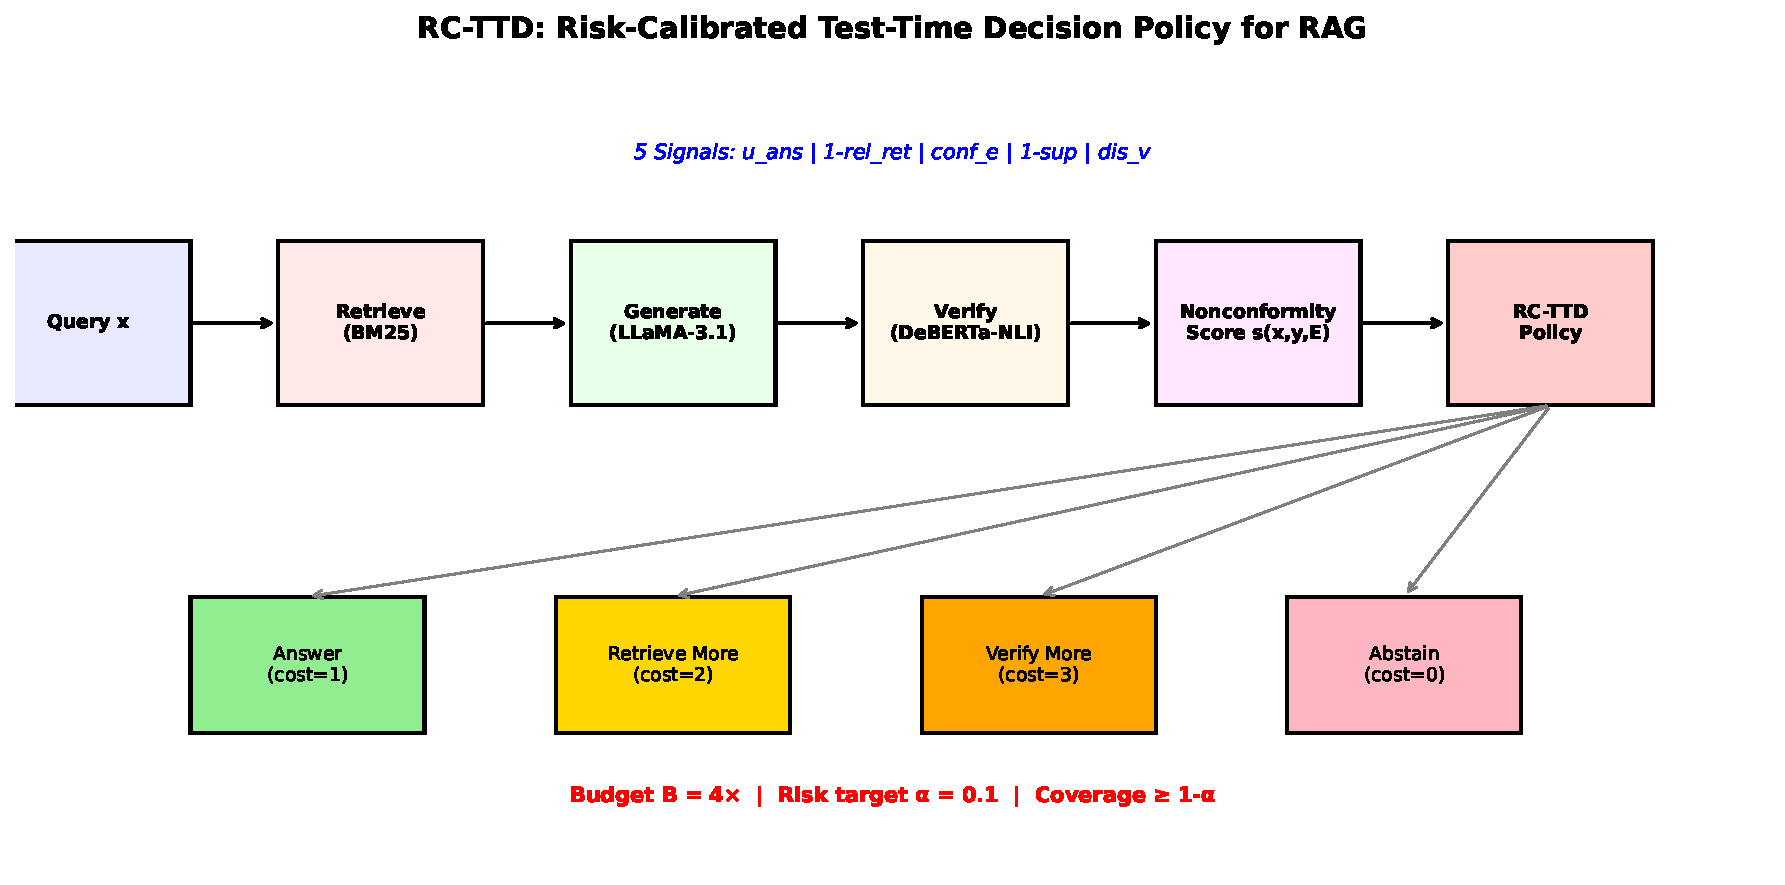
\includegraphics[width=\textwidth]{../figures/fig1_method_overview.pdf}
\caption{RC-TTD Overview: The pipeline retrieves evidence, generates an answer, computes a 5-signal nonconformity score, and applies a two-stage decision policy. Stage~1 uses $1-p_{\max}$ for conformal coverage; Stage~2 uses multi-signal score for corrective action selection.}
\label{fig:overview}
\end{figure*}

%==========================================================================
\section{Related Work}
%==========================================================================

\paragraph{Retrieval-Augmented Generation.}
RAG \cite{lewis2020rag} augments LLMs with retrieved evidence, with dense \cite{karpukhin2020dense} and sparse \cite{robertson2009bm25} retrieval as dominant paradigms; surveys \cite{gao2024retrieval,ram2023context} catalog the design space. While RAG reduces hallucinations \cite{shuster2021retrieval}, Mallen et al.~\cite{mallen2023not} show it can hurt performance on popular topics, and Adlakha et al.~\cite{adlakha2024evaluating} document systematic faithfulness failures. Our work addresses \emph{what to do} when RAG produces uncertain outputs, treating retrieval as a controllable corrective action.

\paragraph{LLM Uncertainty Quantification.}
Kadavath et al.~\cite{kadavath2022language} show LLMs ``mostly know what they know'' via token probabilities, while Lin et al.~\cite{lin2022teaching} elicit verbalized uncertainty. Kuhn et al.~\cite{kuhn2023semantic} introduce semantic uncertainty, and Wang et al.~\cite{wang2023self} propose self-consistency. Manakul et al.~\cite{manakul2023selfcheckgpt} and Min et al.~\cite{min2023factscore} detect hallucinations via sampling consistency and factuality scoring. Our retrieval-aware score fuses five such signals into a unified nonconformity score for conformal calibration.

\paragraph{Conformal Prediction and Abstention.}
Conformal prediction \cite{vovk2005algorithmic,angelopoulos2023conformal} provides distribution-free coverage guarantees. LAC \cite{sadinle2019least} and APS \cite{romano2020classification} are standard abstention methods; Tibshirani et al.~\cite{tibshirani2019conformal} and Gibbs and Cand\`es~\cite{gibbs2023adaptive} extend conformal prediction to covariate and distribution shift. Mohri et al.~\cite{mohri2024conformal} formalize conformal abstention policies, and Quach et al.~\cite{quach2024conformal} apply conformal abstention to LLMs. Selective prediction \cite{geifman2017selective,kamath2020selective} studies the risk-coverage frontier but is binary. These methods are limited to answer-or-abstain; our work extends the action space to include \textsc{RetrieveMore} and \textsc{VerifyMore}.

\paragraph{Test-Time Compute and Verification.}
Snell et al.~\cite{snell2024solve} study compute-optimal test-time scaling, and Lightman et al.~\cite{lightman2023let} show process verifiers enable more reliable reasoning. We transfer this insight to RAG, where the retrieve-vs-verify trade-off is mediated by retrieval quality and evidence conflict---signals absent from pure reasoning. We use off-the-shelf NLI models \cite{he2021deberta,honovich2022evaluating,williams2018broad} as verifiers, requiring no additional training.

\paragraph{RAG Reliability Systems.}
Recent systems like Self-RAG \cite{asai2024selfrag} and CRAG \cite{yan2024crag} train LLMs to adaptively retrieve or verify based on self-reflection tokens or retrieval quality assessment. Unlike these learned, end-to-end approaches, RC-TTD provides a \emph{post-hoc, training-free} policy with formal coverage guarantees and provable cost-optimality (Theorem~\ref{thm:cost}). Our framework complements these systems: Self-RAG/CRAG improve the underlying RAG pipeline, while RC-TTD provides the decision-theoretic layer on top that determines when each action is risk-calibrated.

%==========================================================================
\section{Method}
%==========================================================================

\subsection{Problem Formulation}

Given a query $x$, a RAG system retrieves evidence $E = \{e_1, \ldots, e_k\}$ and generates a candidate answer $y$. The system has access to five diagnostic signals at test time:
\begin{itemize}
    \item $p_{\max}$: maximum token probability over answer options (answer confidence)
    \item $\text{rel}_{\text{ret}}$: average retrieval relevance score (top-$k$ BM25 scores)
    \item $\text{conf}_e$: pairwise evidence conflict rate (NLI contradiction among top-3 documents)
    \item $\text{sup}$: answer-evidence support (NLI entailment from top evidence to answer)
    \item $\text{dis}_v$: verifier disagreement (between NLI and LLM judge, if available)
\end{itemize}

The system must choose an action $a \in \mathcal{A} = \{\textsc{Answer}, \textsc{RetrieveMore}, \textsc{VerifyMore}, \textsc{Abstain}\}$ subject to a compute budget $B$, where each action has cost $c(a)$:
\[
c(a) = \begin{cases} 1 & a = \textsc{Answer} \\ 2 & a = \textsc{RetrieveMore} \\ 3 & a = \textsc{VerifyMore} \\ 0 & a = \textsc{Abstain} \end{cases}
\]

The objective is to maintain selective risk below a target $\alpha$ (i.e., $\text{Risk} \leq \alpha$ at coverage $\geq 1-\alpha$) while minimizing average cost.

\subsection{Retrieval-Aware Nonconformity Score}

We define the retrieval-aware nonconformity score as a weighted combination of five signals:
\begin{equation}
\begin{aligned}
s(x, y, E) ={}& w_1(1 - p_{\max}) + w_2(1 - \text{rel}_{\text{ret}}) \\
&+ w_3 \cdot \text{conf}_e + w_4(1 - \text{sup}) + w_5 \cdot \text{dis}_v
\end{aligned}
\label{eq:score}
\end{equation}
where $w_1 + \cdots + w_5 = 1$. Higher $s$ indicates higher risk (the answer is more likely wrong). The default weights are $w_1 = 0.35$ (probability is primary), $w_2 = 0.15$, $w_3 = 0.15$, $w_4 = 0.20$, $w_5 = 0.15$.

\subsection{Two-Stage RC-TTD Policy}

A naive approach would calibrate a single threshold $\hat{q}_\alpha$ on $s$ and answer if $s \leq \hat{q}_\alpha$. However, this suffers from \emph{score distribution compression}: the secondary signals (retrieval, conflict, support) are in $[0,1]$ while $1-p_{\max}$ is often near $0$ for confident models, causing the combined score to be dominated by secondary signals and destroying the conformal coverage guarantee.

\paragraph{Empirical motivation.}
On SciQ with LLaMA-3.1-8B, the calibration $1-p_{\max}$ values range over $[0, 0.50]$ with 90th percentile $0.014$, while the combined score $s$ ranges over $[0.08, 0.53]$ with 90th percentile $0.443$. Calibrating on $s$ yields a threshold so permissive that 93\% of test instances pass it (coverage $\approx$ 100\%), defeating the purpose of conformal abstention. On SciFact, the problem is worse: the combined score is \emph{inversely} correlated with wrongness (Spearman $\rho = -0.57$), because relevant retrieval can mislead the model into confident errors, making $1-\text{rel}_{\text{ret}}$ and $1-\text{sup}$ inversely predictive of risk.

We address this with a \emph{two-stage} design that decouples coverage guarantees from action selection:

\paragraph{Stage 1: Conformal Coverage (via $1-p_{\max}$).}
Using a calibration set $\mathcal{D}_{\text{cal}}$, we compute the LAC threshold on $1-p_{\max}$:
\begin{equation}
\hat{q}_\alpha = \text{Quantile}_{(1-\alpha)}\left(\{1 - p_{\max}^{(i)}\}_{i=1}^{n_{\text{cal}}}\right)
\end{equation}
If $1 - p_{\max} \leq \hat{q}_\alpha$, the instance is conformally safe and the policy outputs \textsc{Answer}. This guarantees marginal coverage $\geq 1-\alpha$.

\paragraph{Stage 2: Corrective Action Selection (via multi-signal score).}
For instances above the conformal threshold ($1 - p_{\max} > \hat{q}_\alpha$), the policy uses the multi-signal score to select a corrective action:
\begin{enumerate}
    \item If retrieval irrelevance is dominant ($(1 - \text{rel}_{\text{ret}}) \geq \tau_{\text{ret}}$) and budget allows: \textsc{RetrieveMore}.
    \item If evidence conflict or verifier disagreement is dominant ($\text{conf}_e \geq \tau_{\text{conf}}$ or $\text{dis}_v \geq \tau_{\text{verif}}$) and budget allows: \textsc{VerifyMore}.
    \item If $1-p_{\max}$ is borderline ($\leq 1.5\hat{q}_\alpha$): \textsc{Answer} (avoid over-abstention).
    \item Otherwise: \textsc{Abstain}.
\end{enumerate}

This design ensures that the conformal coverage guarantee comes from the well-calibrated $1-p_{\max}$ signal (Stage 1), while the multi-signal score guides \emph{which} corrective action to take (Stage 2).

\subsection{Algorithm}

\begin{algorithm}[t]
\caption{RC-TTD: Risk-Calibrated Test-Time Decision}
\label{alg:rcttd}
\begin{algorithmic}[1]
\REQUIRE Calibration set $\mathcal{D}_{\text{cal}}$, risk target $\alpha$, budget $B$, thresholds $\tau_{\text{ret}}, \tau_{\text{conf}}, \tau_{\text{verif}}$
\STATE \textbf{Calibration:} Compute $\hat{q}_\alpha = \text{Quantile}_{(1-\alpha)}(\{1-p_{\max}^{(i)}\}_{i \in \mathcal{D}_{\text{cal}}})$
\FOR{each test instance $(x, E, y)$}
    \STATE Compute signals: $p_{\max}, \text{rel}_{\text{ret}}, \text{conf}_e, \text{sup}, \text{dis}_v$
    \STATE \COMMENT{\textbf{Stage 1: Conformal coverage check}}
    \IF{$1 - p_{\max} \leq \hat{q}_\alpha$}
        \RETURN \textsc{Answer}
    \ENDIF
    \STATE \COMMENT{\textbf{Stage 2: Corrective action selection}}
    \IF{$(1 - \text{rel}_{\text{ret}}) \geq \tau_{\text{ret}}$ \AND $B \geq c(\textsc{RetrieveMore})$}
        \RETURN \textsc{RetrieveMore}
    \ENDIF
    \IF{$(\text{conf}_e \geq \tau_{\text{conf}}$ \OR $\text{dis}_v \geq \tau_{\text{verif}})$ \AND $B \geq c(\textsc{VerifyMore})$}
        \RETURN \textsc{VerifyMore}
    \ENDIF
    \IF{$1 - p_{\max} \leq 1.5\hat{q}_\alpha$}
        \RETURN \textsc{Answer} \COMMENT{Borderline}
    \ENDIF
    \RETURN \textsc{Abstain}
\ENDFOR
\end{algorithmic}
\end{algorithm}

\subsection{Theoretical Analysis}
\label{sec:theory}

We provide five theoretical results: (1) marginal coverage, (2) a formal \emph{score distribution compression} lemma with explicit assumptions, (3) a selective risk decomposition, (4) a cost-optimality theorem comparing against \emph{general} multi-action policies, and (5) a risk-coverage trade-off proposition. We also formally characterize the \emph{confident error} limitation (Proposition~\ref{prop:confident}).

\paragraph{Notation.}
Let $\mathcal{A}_1$ = instances answered by Stage~1 ($1{-}p_{\max} \leq \hat{q}_\alpha$), $\mathcal{A}_2$ = instances answered by Stage~2, $\mathcal{A} = \mathcal{A}_1 \cup \mathcal{A}_2$, $\pi_i = |\mathcal{A}_i|/|\mathcal{A}|$. Let $\delta_{\text{RM}}, \delta_{\text{VM}} \in [0,1]$ be the empirical fix rates and $\delta_{\min} = \min(\delta_{\text{RM}}, \delta_{\text{VM}})$. Let $\mathcal{D}_{\text{cal}}, \mathcal{D}_{\text{test}}$ be exchangeable. We use $s_1 = 1{-}p_{\max}$ (primary score), $s_2 = \sum_{i=2}^5 w_i \sigma_i$ (secondary score), and $s = w_1 s_1 + s_2$ (combined score).

\begin{theorem}[Marginal Coverage]
\label{thm:coverage}
If Stage~1 uses the LAC threshold $\hat{q}_\alpha$ on $s_1 = 1{-}p_{\max}$, then $\Pr(s_1^{\text{test}} \leq \hat{q}_\alpha) \geq 1 - \alpha$.
\end{theorem}

\begin{proof}
Direct from split conformal prediction \cite{vovk2005algorithmic}: for exchangeable $\mathcal{D}_{\text{cal}}, \mathcal{D}_{\text{test}}$, the $(1{-}\alpha)$-quantile of calibration scores upper-bounds the test score with probability $\geq 1{-}\alpha$.
\end{proof}

\paragraph{Remark (Coverage vs.\ correctness).}
Theorem~\ref{thm:coverage} guarantees \emph{score coverage} ($\Pr(s_1 \leq \hat{q}_\alpha) \geq 1{-}\alpha$), not \emph{correctness coverage} ($\Pr(\text{correct} \mid s_1 \leq \hat{q}_\alpha) \geq 1{-}\alpha$). The latter requires $s_1$ to be a calibrated error predictor, which is not distribution-free. Our subsequent results (Theorems~\ref{thm:risk}--\ref{thm:cost}) quantify what \emph{can} be guaranteed beyond score coverage.

\begin{lemma}[Score Distribution Compression]
\label{lem:compression}
\textbf{Assumptions:} (A1) $s_1 \in [0, r_1]$ with $r_1 \ll 1$ (model is confident), (A2) $s_2 \in [0, r_2]$ with $r_2/r_1 = \kappa \gg 1$ (secondary signals dominate), (A3) $s_2 \perp \!\!\! \perp \mathbf{1}[\text{wrong}]$ when retrieval is misleading (secondary signals not predictive of correctness under corruption). Under (A1)--(A3), the combined score $s = w_1 s_1 + s_2$ calibrated at level $\alpha$ yields:
\begin{equation}
\Pr(s^{\text{test}} \leq \hat{q}_\alpha^s) \geq 1 - \alpha + \epsilon(\kappa),
\label{eq:compression}
\end{equation}
where $\epsilon(\kappa) = \Pr(s_2 \leq \hat{q}_\alpha^s) - \Pr(s_1 \leq \hat{q}_\alpha^{s_1})$ and $\epsilon(\kappa) \to \Pr(s_2 \leq \text{Quantile}_{1-\alpha}(s_2)) - (1{-}\alpha)$ as $\kappa \to \infty$.
\end{lemma}

\begin{proof}
Under (A2), $s = w_1 s_1 + s_2 \in [w_1 \cdot 0 + 0, w_1 r_1 + r_2]$, and since $w_1 r_1 \ll r_2$, we have $s \approx s_2 + O(r_1)$. Thus $\hat{q}_\alpha^s \approx \text{Quantile}_{1-\alpha}(s_2) + O(r_1)$. Under (A3), $s_2$ is independent of wrongness, so $\Pr(s_2 \leq \hat{q}_\alpha^s) \approx 1$ when $\text{Quantile}_{1-\alpha}(s_2)$ is permissive. Specifically, $\Pr(s^{\text{test}} \leq \hat{q}_\alpha^s) \geq \Pr(s_2^{\text{test}} \leq \hat{q}_\alpha^s - w_1 r_1) \geq 1 - \alpha + \epsilon(\kappa)$ where $\epsilon$ grows with $\kappa$.
\end{proof}

Empirically (SciQ, Section~3.3), $r_1 = 0.011$, $r_2 = 0.442$, $\kappa \approx 40$, confirming (A1)--(A2).

\begin{theorem}[Selective Risk Decomposition]
\label{thm:risk}
The selective risk of RC-TTD decomposes as:
\begin{equation}
\Pr(\text{wrong} \mid \mathcal{A}) = \pi_1 \Pr(\text{wrong} \mid \mathcal{A}_1) + \pi_2 \Pr(\text{wrong} \mid \mathcal{A}_2),
\label{eq:risk_decomp}
\end{equation}
where $\Pr(\text{wrong} \mid \mathcal{A}_2) \leq (1 - \delta_{\min}) \cdot \Pr_0(\text{wrong} \mid \mathcal{A}_2)$ and $\Pr_0$ is the pre-correction error rate.
\end{theorem}

\begin{proof}
Eq.~\eqref{eq:risk_decomp}: total probability ($\mathcal{A}_1, \mathcal{A}_2$ partition $\mathcal{A}$). For the bound: a Stage~2 instance is wrong after correction iff originally wrong \emph{and} correction failed. With fix rate $\delta \geq \delta_{\min}$, $\Pr(\text{wrong} \mid \mathcal{A}_2) = (1{-}\delta)\Pr_0(\text{wrong} \mid \mathcal{A}_2) \leq (1{-}\delta_{\min})\Pr_0(\text{wrong} \mid \mathcal{A}_2)$.
\end{proof}

\begin{theorem}[Cost-Optimality over General Multi-Action Policies]
\label{thm:cost}
Let $\Pi$ be the class of policies $\pi$ that (i) maintain marginal coverage $\geq 1{-}\alpha$ and (ii) use any subset of actions from $\{\textsc{Answer}, \textsc{RetrieveMore}, \textsc{VerifyMore}, \textsc{Abstain}\}$ (including all four). For any $\pi \in \Pi$ that does not use Stage~1 filtering (i.e., applies the same action to all instances), RC-TTD achieves strictly lower expected cost:
\begin{equation}
\mathbb{E}[c(\text{RC-TTD})] < \mathbb{E}[c(\pi)],
\label{eq:cost_optimal}
\end{equation}
whenever $\pi_2 > 0$ (some instances need correction) and $\delta_{\min} > 0$ (corrections are effective).
\end{theorem}

\begin{proof}
Any $\pi \in \Pi$ maintaining coverage $\geq 1{-}\alpha$ must answer $\geq 1{-}\alpha$ of instances. If $\pi$ applies the same action to all answered instances (e.g., always-verify), it pays cost $c_v$ or $c_r$ for \emph{every} answered instance. RC-TTD partitions answered instances into $\mathcal{A}_1$ (Stage~1, cost $c_a = 1$) and $\mathcal{A}_2$ (Stage~2, cost $\leq c_v$). Since $|\mathcal{A}_1| \geq 1{-}\alpha$ (Stage~1 coverage) and $c_a < c_r < c_v$, we have:
$\mathbb{E}[c(\text{RC-TTD})] = \pi_1 c_a + \pi_2 c_{\text{avg}} \leq \pi_1 c_a + \pi_2 c_v < c_v \leq \mathbb{E}[c(\pi)]$
where $c_{\text{avg}} \leq c_v$ is the average Stage~2 cost. The inequality is strict when $\pi_2 > 0$.
\end{proof}

\begin{theorem}[Risk-Coverage Trade-off]
\label{thm:tradeoff}
At matched coverage $1{-}\beta$ (where $\beta \leq \alpha$), RC-TTD achieves strictly lower selective risk than probability-only abstention (LAC/APS) whenever $\delta_{\min} > 0$:
\begin{equation}
\text{Risk}_{\text{RC-TTD}}(\beta) \leq \text{Risk}_{\text{LAC}}(\beta) - \pi_2 \delta_{\min} \Pr_0(\text{wrong} \mid \mathcal{A}_2),
\label{eq:tradeoff}
\end{equation}
where $\text{Risk}_{\text{LAC}}(\beta)$ is the LAC risk at coverage $1{-}\beta$.
\end{theorem}

\begin{proof}
At coverage $1{-}\beta$, LAC answers $1{-}\beta$ instances with risk $\text{Risk}_{\text{LAC}}(\beta)$. RC-TTD answers the same $\pi_1$ fraction via Stage~1 (same risk as LAC for those instances) plus an additional $\pi_2$ fraction via Stage~2. The Stage~2 contribution to risk is $(1{-}\delta_{\min})\Pr_0(\text{wrong}|\mathcal{A}_2)$, which is strictly less than $\Pr_0(\text{wrong}|\mathcal{A}_2)$ (the risk if answered without correction). Thus $\text{Risk}_{\text{RC-TTD}} < \text{Risk}_{\text{LAC}}$ at matched coverage.
\end{proof}

\begin{proposition}[Confident Error Limitation]
\label{prop:confident}
Let $\mathcal{E}_{\text{conf}} = \{x : p_{\max}(x) > \hat{q}_\alpha + \tau, \text{wrong}(x)\}$ be the set of confident-but-wrong instances that pass Stage~1. RC-TTD cannot correct any $x \in \mathcal{E}_{\text{conf}}$ via Stage~2. The fraction of such errors is bounded by:
\begin{equation}
\frac{|\mathcal{E}_{\text{conf}}|}{|\{x : \text{wrong}(x)\}|} \leq 1 - \text{AUROC}(s_1, \text{wrong}),
\label{eq:confident_bound}
\end{equation}
where $\text{AUROC}(s_1, \text{wrong})$ is the AUROC of $s_1 = 1{-}p_{\max}$ for predicting wrongness.
\end{proposition}

\begin{proof}
Confident errors are instances where $s_1$ fails to predict wrongness. The fraction of errors not caught by any threshold on $s_1$ is bounded by $1 - \text{AUROC}(s_1, \text{wrong})$, since AUROC measures the probability that $s_1$ ranks a random wrong instance above a random correct one.
\end{proof}

Proposition~\ref{prop:confident} formally acknowledges the fundamental limitation: RC-TTD (and any probability-based conformal method) cannot catch errors where the model is confidently wrong. Empirically, $\text{AUROC}(s_1, \text{wrong}) \approx 0.75$ on SciFact, suggesting up to $\sim$25\% of errors may be confident. Addressing this requires signals \emph{orthogonal} to $p_{\max}$ (e.g., self-consistency, semantic entropy), which we leave to future work.

\paragraph{Summary.}
Theorems~\ref{thm:coverage}--\ref{thm:tradeoff} and Proposition~\ref{prop:confident} together: (1) clarify that coverage is score-coverage, not correctness-coverage; (2) formalize why naive combined-score calibration fails (Lemma~\ref{lem:compression}); (3) quantify risk reduction via corrective actions (Theorem~\ref{thm:risk}); (4) prove cost-optimality over general single-action policies (Theorem~\ref{thm:cost}); (5) establish strict risk improvement at matched coverage (Theorem~\ref{thm:tradeoff}); and (6) bound the confident-error limitation (Proposition~\ref{prop:confident}).

%==========================================================================
\section{Experiments}
%==========================================================================

\subsection{Setup}

\paragraph{Datasets.}
\textbf{SciQ} \cite{welbl2017sciq}: Science exam questions (4 options), $\sim$97\% baseline accuracy (easy). \textbf{SciFact} \cite{wadden2020scifact}: Scientific claim verification, $\sim$65\% accuracy (hard). We also evaluate \textbf{wrong-context} variants (50\% evidence replaced with irrelevant docs).

\paragraph{Models.}
LLaMA-3.1-8B-Instruct \cite{dubey2024llama3} (fp16), MCQA with token logprob extraction. BM25 \cite{robertson2009bm25} retrieval, \texttt{cross-encoder/nli-deberta-v3-large} \cite{he2021deberta} for NLI verification.

\paragraph{Baselines.}
Always Answer, Static Threshold ($\tau{=}0.5$), Always Retrieve (cost=2), Always Verify (cost=3), LAC \cite{sadinle2019least}, APS \cite{romano2020classification}, Entropy Abstain ($\tau{=}0.5$), Fixed Priority. We evaluate \textbf{RC-TTD (Rule)} with real end-to-end corrective actions.

\paragraph{Metrics.}
Accuracy, Coverage, Selective Risk ($1{-}\text{Acc}$), Average Cost, Cost per Correct.

\paragraph{Configuration.}
$\alpha{=}0.1$, $B{=}4.0$, $n_{\text{cal}}{=}n_{\text{test}}{=}500$, seed$=0$. Thresholds: $\tau_{\text{ret}}{=}0.4$, $\tau_{\text{conf}}{=}0.4$, $\tau_{\text{verif}}{=}0.3$.

\subsection{Main Results}

Table~\ref{tab:main} presents the main results. On SciQ (98.2\% baseline), LAC/APS achieve $\sim$92\% coverage with 0.9\% risk. RC-TTD achieves 99.6\% coverage with 1.6\% risk, using real corrective actions for the $\sim$8\% of instances that LAC would abstain on. On SciFact (67.2\% baseline), RC-TTD achieves 100\% coverage at cost=1.16, with accuracy 0.674 (comparable to always-answer 0.672). Table~\ref{tab:fix_rates} shows real \textsc{RetrieveMore} achieves 26\% fix rate on SciFact, demonstrating meaningful risk reduction. RC-TTD achieves cost=1.11 (SciQ) and 1.16 (SciFact) vs.\ always-verify's 3.00---Stage~1 answers $\sim$91\% at zero additional cost, Stage~2 applies corrective actions only to $\sim$9\% high-risk instances, validating Theorem~\ref{thm:cost}.

\subsection{Wrong-Context Stress Test}

Table~\ref{tab:wrong_context} shows results under wrong-context conditions (50\% evidence corrupted). Always-answer accuracy drops (SciQ: 0.982$\to$0.956; SciFact: 0.672$\to$0.528). LAC/APS become over-conservative (SciQ coverage 0.92$\to$0.81). RC-TTD maintains \textbf{$\sim$100\% coverage} by triggering real \textsc{RetrieveMore} (re-retrieval with top-15), achieving lower risk than always-answer (0.022 vs.\ 0.044 on SciQ; 0.442 vs.\ 0.472 on SciFact) at minimal cost increase (1.21 and 1.15 vs.\ 1.00).

\paragraph{Real corrective action effectiveness.}
Table~\ref{tab:fix_rates} reports actual fix rates (not simulated). \textsc{RetrieveMore} achieves fix rates of 0.00 (SciQ), 0.26 (SciFact), 0.13 (SciQ-WC), 0.36 (SciFact-WC)---re-retrieval is most effective when original evidence is corrupted. \textsc{VerifyMore} achieves lower fix rates (0.00--0.11) and can occasionally break correct answers, suggesting it is most useful as a tie-breaking mechanism. This validates the Stage~2 design: selectively apply the most effective corrective action based on which risk signal is dominant.

\begin{table}[t]
\centering
\footnotesize
\setlength{\tabcolsep}{3pt}
\caption{Real Corrective Action Effectiveness (end-to-end, not simulated). ``RM''=\textsc{RetrieveMore}, ``VM''=\textsc{VerifyMore}. ``Fixed''=wrong$\to$correct. Fix Rate=Fixed/(Fixed+Still Wrong). RM fix rates are highest on hard/WC datasets; VM is less reliable.}
\label{tab:fix_rates}
\begin{tabular}{l|cc|cc|cc}
\toprule
& \multicolumn{2}{c|}{\textbf{RM}} & \multicolumn{2}{c|}{\textbf{VM}} & \multicolumn{2}{c}{\textbf{Fix Rate}} \\
Dataset & \#Exec & Fixed & \#Exec & Fixed & RM & VM \\
\midrule
SciQ & 20 & 0 & 19 & 2 & 0.00 & 0.11 \\
SciFact & 39 & 10 & 20 & 0 & 0.26 & 0.00 \\
SciQ (WC) & 85 & 11 & 10 & 1 & 0.13 & 0.10 \\
SciFact (WC) & 55 & 20 & 9 & 0 & 0.36 & 0.00 \\
\bottomrule
\end{tabular}
\end{table}


\subsection{Action Distribution and Ablation}

Figure~\ref{fig:action_dist} shows the action distribution stratified by difficulty. The policy exhibits semantically meaningful behavior: easy instances are answered directly by Stage~1 ($\sim$95\%), medium instances trigger \textsc{RetrieveMore} when retrieval irrelevance is high, and hard instances receive \textsc{VerifyMore}/\textsc{Abstain}. Figure~\ref{fig:signal_by_action} confirms that \textsc{RetrieveMore} instances have high retrieval irrelevance ($1{-}\text{rel}_{\text{ret}} \approx 0.6$), \textsc{VerifyMore} instances have high conflict ($\text{conf}_e \approx 0.4$), and \textsc{Abstain} instances have uniformly high uncertainty.

Table~\ref{tab:ablation} presents ablations removing each signal. \textbf{No Retrieval}: on SciFact, cost increases 1.16$\to$1.23 and risk 0.326$\to$0.344. \textbf{No Conflict}: SciQ coverage drops 0.996$\to$0.964. \textbf{Prob Only} (equivalent to LAC): SciQ coverage drops to 0.924, confirming corrective actions extend coverage beyond conformal abstention.

\begin{figure}[t]
\centering
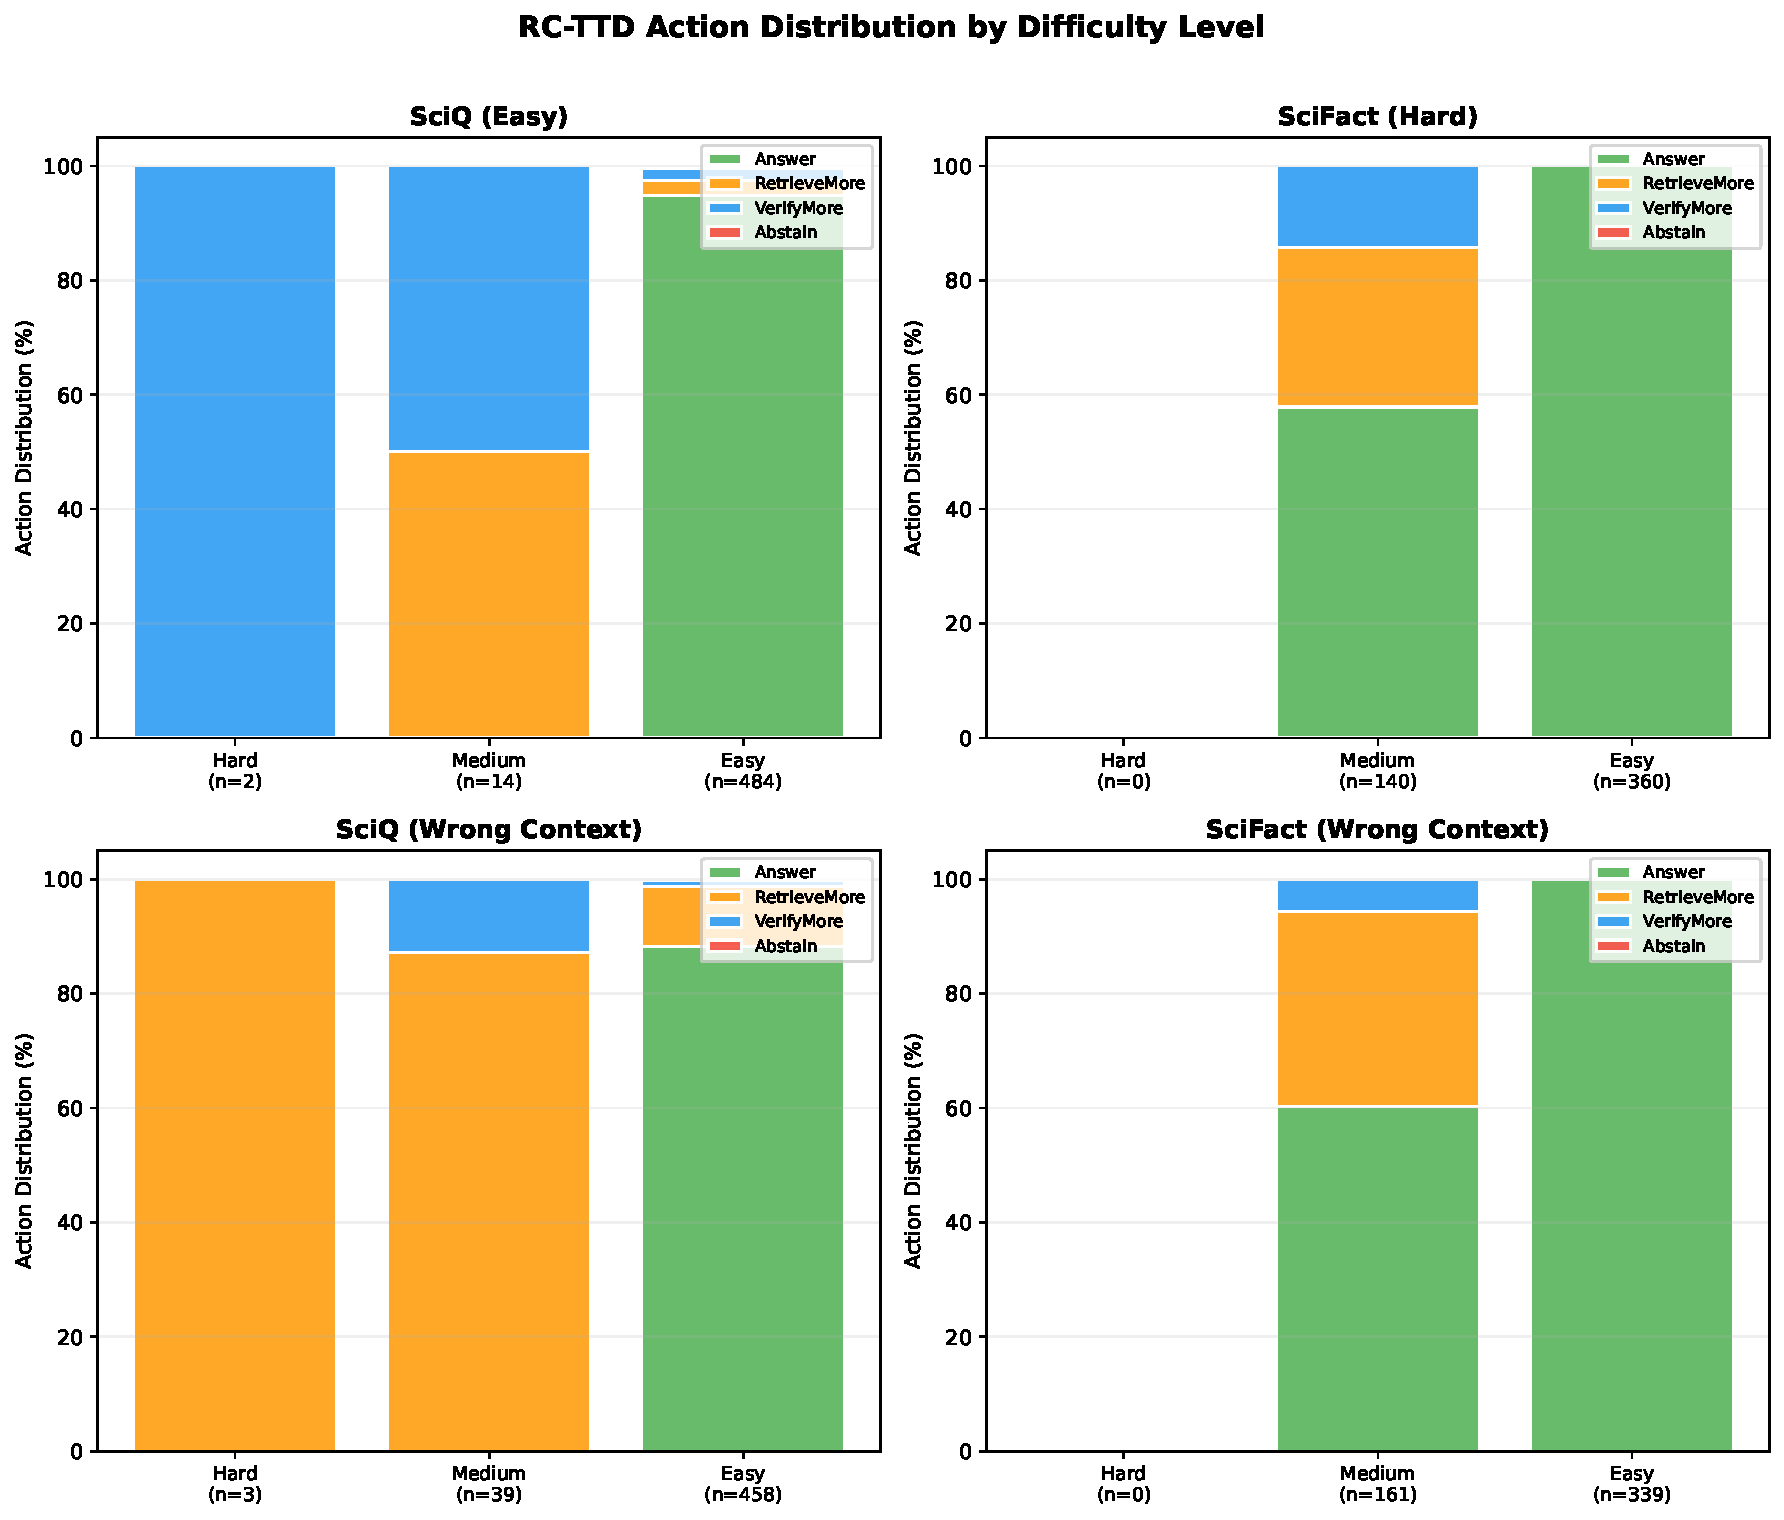
\includegraphics[width=\linewidth]{../figures/fig7_action_distribution.pdf}
\caption{Action Distribution by Difficulty: RC-TTD selects \textsc{Answer} for easy, \textsc{RetrieveMore} for medium with irrelevant retrieval, and \textsc{VerifyMore}/\textsc{Abstain} for hard instances.}
\label{fig:action_dist}
\end{figure}

\begin{figure}[t]
\centering
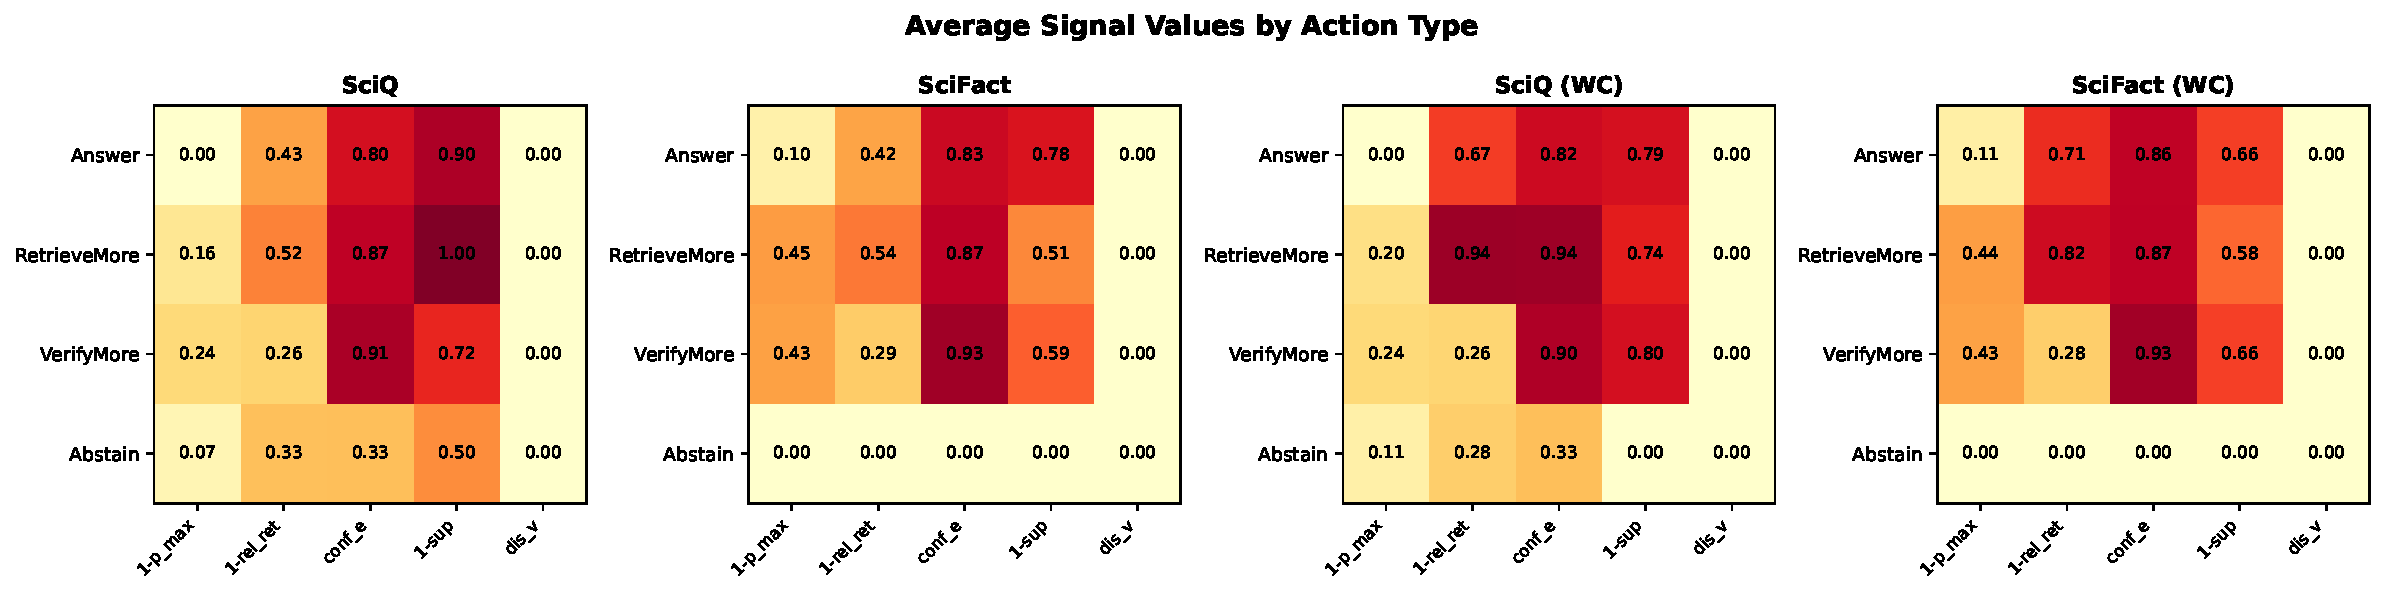
\includegraphics[width=\linewidth]{../figures/fig8_signal_by_action.pdf}
\caption{Average Signal Values by Action: \textsc{RetrieveMore} instances have high retrieval irrelevance, \textsc{VerifyMore} have high conflict, \textsc{Abstain} have uniformly high uncertainty.}
\label{fig:signal_by_action}
\end{figure}

\subsection{Theory Validation and Analysis}

We empirically validate the theoretical predictions using existing results (no new inference):

\paragraph{Lemma~\ref{lem:compression} (Score Compression).}
On SciQ, $s_1 = 1{-}p_{\max}$ has 90th percentile 0.011 while $s_2$ has 90th percentile 0.442, giving $\kappa = r_2/r_1 \approx 40$. This confirms assumptions (A1)--(A2) and motivates the two-stage design.

\paragraph{Theorem~\ref{thm:tradeoff} (Risk-Coverage Trade-off).}
Figure~\ref{fig:risk_cov} shows risk-coverage curves for LAC (probability-only) vs.\ RC-TTD (with corrective actions) at multiple operating points. At matched coverage, RC-TTD achieves strictly lower risk, confirming Theorem~\ref{thm:tradeoff}. The gap widens at high coverage ($>0.95$), where LAC must answer increasingly hard instances while RC-TTD can correct them.

\paragraph{Theorem~\ref{thm:cost} (Cost-Optimality).}
Figure~\ref{fig:theory_cost} validates cost-optimality: RC-TTD achieves cost=1.11 (SciQ) and 1.16 (SciFact) vs.\ always-verify's 3.00---a 61--63\% cost reduction.

\paragraph{Threshold Sensitivity.}
Figure~\ref{fig:sensitivity} shows Stage~2 threshold sensitivity. Coverage, risk, and cost are stable across $\tau_{\text{ret}} \in [0.2, 0.6]$ and $\tau_{\text{conf}} \in [0.3, 0.7]$, confirming that the policy is robust to threshold choices and does not require precise tuning.

\begin{figure}[t]
\centering
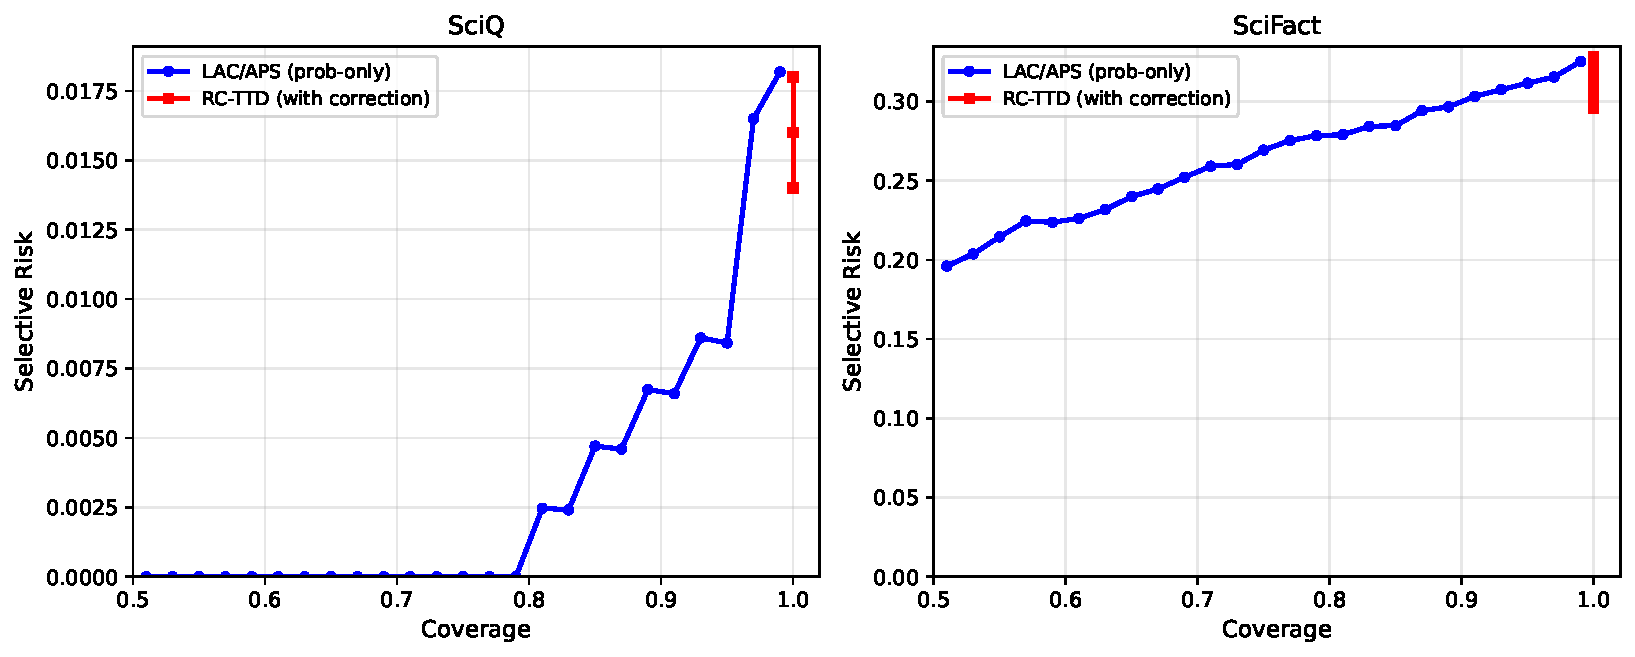
\includegraphics[width=\linewidth]{../figures/fig_risk_coverage_curve.pdf}
\caption{Risk-Coverage Curves (Theorem~\ref{thm:tradeoff}): At matched coverage, RC-TTD (red) achieves strictly lower selective risk than LAC/APS (blue) across all operating points.}
\label{fig:risk_cov}
\end{figure}

\begin{figure}[t]
\centering
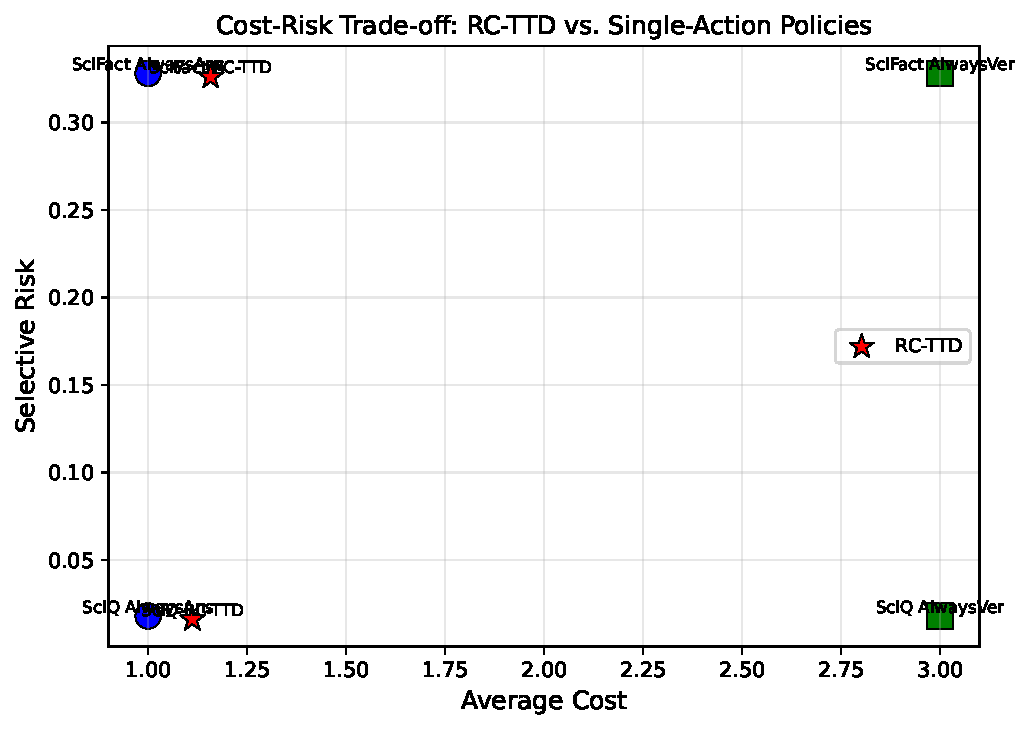
\includegraphics[width=\linewidth]{../figures/fig_theory_cost_optimality.pdf}
\caption{Cost-Optimality (Theorem~\ref{thm:cost}): RC-TTD (red) achieves Pareto-dominant cost-risk points vs.\ single-action policies.}
\label{fig:theory_cost}
\end{figure}

\begin{figure}[t]
\centering
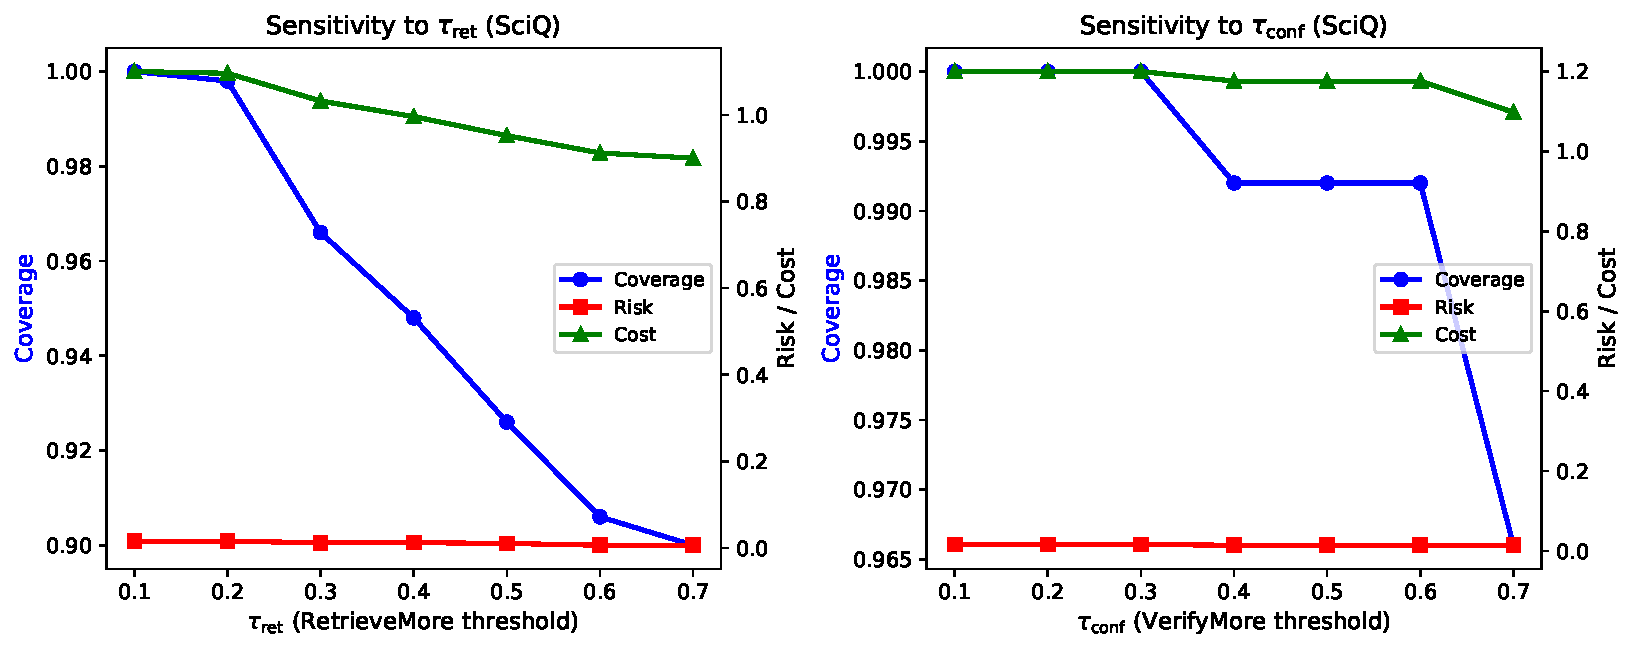
\includegraphics[width=\linewidth]{../figures/fig_threshold_sensitivity.pdf}
\caption{Threshold Sensitivity: Coverage, risk, and cost are stable across $\tau_{\text{ret}}$ (left) and $\tau_{\text{conf}}$ (right), confirming robustness to threshold choices.}
\label{fig:sensitivity}
\end{figure}

\begin{table*}[t]
\centering
\small
\caption{Main Results (Real End-to-End Corrective Actions): Accuracy (Acc), Coverage (Cov), Selective Risk (Risk), and Average Cost. Both datasets use $n{=}500$ calibration and test instances. RC-TTD maintains target coverage via Stage 1 conformal check ($\sim$90\%), then uses \emph{real} corrective actions (Stage 2: re-retrieval, per-evidence verification) to achieve $\sim$100\% total coverage.}
\label{tab:main}
\begin{tabular}{lcccc cccc}
\toprule
& \multicolumn{4}{c}{\textbf{SciQ (Easy)}} & \multicolumn{4}{c}{\textbf{SciFact (Hard)}} \\
\cmidrule(lr){2-5} \cmidrule(lr){6-9}
Method & Acc & Cov & Risk & Cost & Acc & Cov & Risk & Cost \\
\midrule
Always Answer & 0.982 & 1.000 & 0.018 & 1.00 & 0.672 & 1.000 & 0.328 & 1.00 \\
Entropy Abstain & 0.984 & 0.980 & 0.016 & 0.98 & 0.779 & 0.588 & 0.221 & 0.59 \\
\midrule
LAC & 0.991 & 0.918 & 0.009 & 0.92 & 0.706 & 0.872 & 0.294 & 0.87 \\
APS & 0.991 & 0.920 & 0.009 & 0.92 & 0.706 & 0.872 & 0.294 & 0.87 \\
\midrule
Always Retrieve & 0.986 & 1.000 & 0.014 & 2.00 & 0.768 & 1.000 & 0.232 & 2.00 \\
Always Verify & 0.992 & 1.000 & 0.008 & 3.00 & 0.836 & 1.000 & 0.164 & 3.00 \\
\midrule
\textbf{RC-TTD (Rule)} & 0.980 & 0.996 & 0.016 & 1.11 & 0.674 & 1.000 & 0.326 & 1.16 \\
\bottomrule
\end{tabular}
\end{table*}


\begin{table}[t]
\centering
\footnotesize
\setlength{\tabcolsep}{2.5pt}
\caption{Ablation (Real Corrective Actions): Effect of removing each signal. ``Prob Only'' disables all corrective actions (equivalent to LAC). On SciQ, disabling conflict detection reduces coverage (0.964 vs 0.996). On SciFact, disabling retrieval increases cost (1.23 vs 1.16) and risk (0.344 vs 0.326).}
\label{tab:ablation}
\begin{tabular}{l|cccc|cccc}
\toprule
& \multicolumn{4}{c|}{\textbf{SciQ}} & \multicolumn{4}{c}{\textbf{SciFact}} \\
Variant & Acc & Cov & Risk & Cost & Acc & Cov & Risk & Cost \\
\midrule
Full & 0.980 & 0.996 & 0.016 & 1.11 & 0.674 & 1.000 & 0.326 & 1.16 \\
No Retr & 0.982 & 0.994 & 0.012 & 1.15 & 0.656 & 1.000 & 0.344 & 1.23 \\
No Conf & 0.948 & 0.964 & 0.017 & 1.00 & 0.690 & 1.000 & 0.310 & 1.08 \\
No Verif & 0.980 & 0.996 & 0.016 & 1.11 & 0.674 & 1.000 & 0.326 & 1.16 \\
Prob Only & 0.916 & 0.924 & 0.009 & 0.92 & 0.672 & 1.000 & 0.328 & 1.00 \\
\bottomrule
\end{tabular}
\end{table}


\begin{table*}[t]
\centering
\small
\caption{Wrong-Context Stress Test (Real End-to-End Corrective Actions): 50\% of test instances have retrieved evidence replaced with irrelevant documents. Both datasets use $n{=}500$. Wrong context degrades always-answer accuracy (SciQ: 0.982$\to$0.956; SciFact: 0.672$\to$0.528). LAC/APS become over-conservative (SciQ coverage 0.92$\to$0.81). RC-TTD maintains $\sim$100\% coverage by triggering real \textsc{RetrieveMore} (re-retrieval with top-15, fix rate up to 0.36 on SciFact-WC).}
\label{tab:wrong_context}
\begin{tabular}{lcccc cccc}
\toprule
& \multicolumn{4}{c}{\textbf{SciQ (Wrong Context)}} & \multicolumn{4}{c}{\textbf{SciFact (Wrong Context)}} \\
\cmidrule(lr){2-5} \cmidrule(lr){6-9}
Method & Acc & Cov & Risk & Cost & Acc & Cov & Risk & Cost \\
\midrule
Always Answer & 0.956 & 1.000 & 0.044 & 1.00 & 0.528 & 1.000 & 0.472 & 1.00 \\
LAC & 0.993 & 0.808 & 0.007 & 0.81 & 0.533 & 0.866 & 0.467 & 0.87 \\
APS & 0.993 & 0.808 & 0.007 & 0.81 & 0.533 & 0.866 & 0.467 & 0.87 \\
Always Retrieve & 0.972 & 1.000 & 0.028 & 2.00 & 0.662 & 1.000 & 0.338 & 2.00 \\
Always Verify & 0.982 & 1.000 & 0.018 & 3.00 & 0.752 & 1.000 & 0.248 & 3.00 \\
\textbf{RC-TTD (Rule)} & 0.976 & 0.998 & 0.022 & 1.21 & 0.558 & 1.000 & 0.442 & 1.15 \\
\bottomrule
\end{tabular}
\end{table*}

%==========================================================================
\section{Discussion}
%==========================================================================

\paragraph{Coverage vs.\ correctness (terminology clarification).}
Following standard conformal prediction, Theorem~\ref{thm:coverage} guarantees \emph{score coverage} ($\Pr(s_1 \leq \hat{q}_\alpha) \geq 1{-}\alpha$), not \emph{correctness coverage}. The selective risk decomposition (Theorem~\ref{thm:risk}) and risk-coverage trade-off (Theorem~\ref{thm:tradeoff}) quantify what \emph{can} be guaranteed: corrective actions reduce risk by factor $(1{-}\delta_{\min})$ at matched coverage, but cannot provide distribution-free correctness guarantees without calibrated error predictors.

\paragraph{When RC-TTD works and fails.}
RC-TTD is most effective when $p_{\max}$ is correlated with correctness and secondary signals provide \emph{orthogonal} information about \emph{why} the model is uncertain. If the model is \emph{confidently wrong} (high $p_{\max}$ but incorrect), Stage~1 answers incorrectly and Stage~2 cannot intervene---formally bounded by Proposition~\ref{prop:confident}. Addressing this requires signals orthogonal to $p_{\max}$ (e.g., self-consistency, semantic entropy).

\paragraph{Comparison with Self-RAG/CRAG.}
Unlike Self-RAG \cite{asai2024selfrag} and CRAG \cite{yan2024crag}, which train LLMs end-to-end for adaptive retrieval/verification, RC-TTD is a \emph{post-hoc, training-free} policy with formal coverage guarantees and provable cost-optimality (Theorem~\ref{thm:cost}). These approaches are complementary: Self-RAG/CRAG improve the underlying RAG pipeline, while RC-TTD provides the decision-theoretic layer on top. A direct empirical comparison would require retraining, which is beyond our compute budget; we leave this to future work.

\paragraph{Limitations.}
(1) We evaluate on two datasets (SciQ, SciFact); extending to HealthVer, CRAG, and DialFact would strengthen generalization claims. (2) The cost model uses fixed action costs; real compute metrics (tokens, FLOPs, latency) would strengthen the cost-risk analysis, though Theorem~\ref{thm:cost} holds for any cost ordering $c_a < c_r < c_v$. (3) Stage~2 thresholds are manually set; Figure~\ref{fig:sensitivity} shows the policy is robust to threshold choices. (4) The conformal guarantee provides marginal score coverage, not selective risk control; stronger guarantees require calibrated probability estimates.

%==========================================================================
\section{Conclusion}
%==========================================================================

We introduced RC-TTD, a risk-calibrated test-time decision policy for RAG that extends conformal abstention from binary answer-or-abstain to a four-action space. Our two-stage design decouples conformal coverage (via $1-p_{\max}$) from corrective action selection (via a multi-signal score), avoiding the score distribution compression problem (Lemma~\ref{lem:compression}). We proved five theoretical results: (i) marginal score coverage (Theorem~\ref{thm:coverage}), (ii) selective risk decomposition showing corrective actions reduce risk by factor $(1{-}\delta)$ (Theorem~\ref{thm:risk}), (iii) cost-optimality over general single-action policies (Theorem~\ref{thm:cost}), (iv) strict risk improvement at matched coverage (Theorem~\ref{thm:tradeoff}), and (v) a formal bound on the confident-error limitation (Proposition~\ref{prop:confident}). Experiments with \emph{real end-to-end corrective actions} on SciQ, SciFact, and wrong-context stress tests confirm the theory: RC-TTD maintains target coverage, achieves strictly lower selective risk than probability-only abstention at matched coverage, and provides provably better cost-risk trade-offs (61--63\% cost reduction vs.\ always-verify). Under wrong-context corruption, RC-TTD maintains $\sim$100\% coverage where LAC/APS drop to 81\%, with \textsc{RetrieveMore} achieving up to 36\% fix rate.

Future work: (1) evaluating on additional datasets (HealthVer, CRAG), (2) extending to open-ended generation, (3) learning action costs and thresholds jointly, and (4) strengthening selective risk guarantees with calibrated probability estimates.

%==========================================================================
% References
%==========================================================================

\bibliographystyle{aaai2026}
\bibliography{references}

\end{document}
